\documentclass[conference]{IEEEtran}
\IEEEoverridecommandlockouts
% The preceding line is only needed to identify funding in the first footnote. If that is unneeded, please comment it out.
\usepackage{cite}
\usepackage{url}
\usepackage{etoolbox}
\usepackage{amsmath,amssymb,amsfonts}
\usepackage{algorithmic}
\usepackage{graphicx}
\usepackage{textcomp}
\usepackage{xcolor}
\usepackage{booktabs}   % For standard academic table rules (\toprule, \midrule, \bottomrule)
\usepackage{multirow}   % For multirow cell spanning
\usepackage{array}      % For enhanced table formatting
\usepackage{siunitx}    % Optional but recommended for handling numeric formatting
\usepackage[utf8]{inputenc}
\usepackage{newunicodechar}
\newunicodechar{−}{\textminus}
\newunicodechar{≥}{\geq}
\usepackage{orcidlink}
%\usepackage{hyperref}
\patchcmd{\IEEEkeywords}{Index Terms}{Keywords}{}{}

% Float placement optimization to ensure 4-page layout + 1-page references
\setcounter{dbltopnumber}{2}
\renewcommand{\topfraction}{0.95}
\renewcommand{\dbltopfraction}{0.95}
\renewcommand{\textfraction}{0.05}
\renewcommand{\floatpagefraction}{0.8}
\renewcommand{\dblfloatpagefraction}{0.8}
\setlength{\textfloatsep}{5pt plus 2pt minus 2pt}
\setlength{\floatsep}{5pt plus 2pt minus 2pt}
\setlength{\intextsep}{5pt plus 2pt minus 2pt}
\setlength{\dbltextfloatsep}{5pt plus 2pt minus 2pt}
\setlength{\dblfloatsep}{5pt plus 2pt minus 2pt}
\setlength{\abovecaptionskip}{3pt}
\setlength{\belowcaptionskip}{2pt}

\def\BibTeX{{\rm B\kern-.05em{\sc i\kern-.025em b}\kern-.08em
    T\kern-.1667em\lower.7ex\hbox{E}\kern-.125emX}}
\begin{document}
\title{EEG-BASED MIND WANDERING CHARACTERIZATION USING MULTI-DOMAIN FEATURES\vspace{-4mm}
% \title{DECODING MIND WANDERING THROUGH NEURAL DYNAMICS AND MULTIDOMAIN FEATURES\vspace{-4mm}
}

\author{
\IEEEauthorblockN{
Shubham\textsuperscript{1}\,\href{https://orcid.org/0009-0002-8673-0321}{\orcidlink{0009-0002-8673-0321}},
Rishwanth JVK\textsuperscript{2}\,\href{https://orcid.org/0009-0004-3552-352X}{\orcidlink{0009-0004-3552-352X}},
Amita Giri\textsuperscript{1}\,\href{https://orcid.org/0000-0002-4564-0269}{\orcidlink{0000-0002-4564-0269}}
}
\IEEEauthorblockA{
\textsuperscript{1}\textit{Department of Electronics and Communication Engineering, Indian Institute of Technology, Roorkee, 247667, India}\\
\textsuperscript{2}\textit{Department of Computer Science and Engineering, Manipal Institute of Technology, Karnataka, 576104, India}\\
Emails: shubham1@ece.iitr.ac.in, rishwanthjvk06@gmail.com, amita.giri@ece.iitr.ac.in
}
}
\maketitle 
\begin{abstract}
Mind wandering (MW)---a shift of attention from an ongoing task toward internally generated thought---is a pervasive cognitive state associated with attentional lapses and reduced task performance. Its accurate detection is therefore important for applications in attention monitoring, education, and cognitive-state-aware systems. Prior EEG studies on mind wandering have largely relied on a single feature domain---and have been validated on a single dataset with one experimental paradigm and channel configuration. This narrow scope leaves open two key questions: (1) whether MW-related neural signatures generalize across task designs and recording setups, and (2) whether specific feature families or frequency bands carry inherently greater discriminative value than others. To address these questions, we propose an integrated EEG framework that jointly characterizes MW by examining feature-family importance alongside frequency-band and within-epoch temporal dynamics across MW and Focus states. The framework is evaluated on two publicly available datasets differing in channel density and experimental paradigm. \textcolor{blue}{Frequency-band analysis demonstrated that $\alpha$ and $\theta$ oscillations contributed the highest overall feature importance across both datasets (jointly accounting for $\sim$65\% of aggregate importance), while $\beta$, $\gamma$, and $\delta$ bands provided complementary discriminative contributions.} Feature-family analysis identified Hjorth parameters as the most informative per feature across both datasets, while functional connectivity contributed minimally. Systematic ablation confirmed spectral features as most critical for discrimination overall, though the most informative individual feature family and frequency band varied across datasets.

\end{abstract}

\textbf{\textit{Keywords---}\textit{Mind wandering}, \textit{EEG}, \textit{Spectral Features}, \textit{Nonlinear Features}, \textit{Cognitive State Classification}.}
 
\section{Introduction}

\textcolor{blue}{Mind wandering (MW) refers to a cognitive state characterized by a shift of attention from an ongoing task toward internally generated thoughts \cite{smallwood2013restless,killingsworth2010wandering}. As a pervasive mental state associated with attentional lapses and reduced task performance \cite{killingsworth2010wandering}, its accurate detection is important for attention monitoring, education, and cognitive-state-aware systems. Internally directed cognition has been linked to default mode network (DMN) dynamics \cite{raichle2001default} and its interactions with executive control networks \cite{christoff2016mind}. Sustained-attention paradigms, such as meditation and breath-focus tasks, provide controlled experimental frameworks for investigating MW by requiring continuous attentional regulation and meta-awareness \cite{lutz2008attention,tang2015neuroscience,cahn2013meditation}. With its millisecond temporal resolution, electroencephalography (EEG) is uniquely suited for capturing oscillatory transitions between sustained focus and spontaneous MW \cite{KAM2022119372,rodlarios}.}

\textcolor{blue}{Prior EEG studies on MW have largely relied on single feature domains---predominantly static band power in low-frequency $\alpha$ and $\theta$ oscillations \cite{KAM2022119372,rodlarios} or high-frequency activity \cite{berkovich2012mindfulness}, alongside isolated complexity metrics \cite{lu2022nonlinear}---evaluated with standard classifiers \cite{jin2020distinguishing,compton2019wandering,hosseini2019deep}. Crucially, nearly all existing investigations were validated on a single dataset with one experimental paradigm and montage. This narrow scope leaves open two key questions: (1) whether MW-related neural signatures generalize across task designs and recording setups, and (2) whether specific feature families or frequency bands carry inherently greater discriminative value than others. Furthermore, conventional feature-importance evaluations assess raw aggregate contributions without accounting for feature-space dimensionality or within-epoch temporal dynamics.}

\textcolor{blue}{To address these questions, we propose an integrated EEG framework that jointly characterizes MW by examining feature-family importance alongside frequency-band and within-epoch temporal dynamics across MW and Focus states. Considering the nonstationary nature of EEG, the framework unifies spectral, time-domain, Hjorth dynamic, entropy, envelope, and phase-locking connectivity features across five frequency bands ($\delta$, $\theta$, $\alpha$, $\beta$, $\gamma$). We evaluate on two publicly available datasets differing in channel density and task design: a 19-channel standard montage using a breath-focused meditation probe design \cite{rodlarios}, and a 64-channel high-density montage employing an event-locked reverse breath-counting paradigm \cite{grandchamp2014oculometric}. Cross-validation incorporating both stratified pooled and subject-session grouped schemes ensures rigorous evaluation without data leakage.}

\textcolor{blue}{Our empirical findings provide systematic answers to both questions. Evaluating total frequency-band contributions revealed that low-frequency ($\alpha$ and $\theta$) oscillations contribute the highest overall importance across both datasets, while high-frequency and $\delta$ bands provide complementary discriminative value. Feature-family analysis identified Hjorth parameters as the most informative per feature across both datasets, while functional connectivity contributed minimally. Temporal modeling uncovered within-epoch dynamics masked by static averages, including progressive $\delta$ accumulation reflecting vigilance degradation and state-divergent $\beta$ trends. Finally, ablation confirmed spectral features as most critical overall, though the most informative individual domain varied across datasets. Together, these results provide a unified characterization of MW dynamics, showing that robust decoding blends universal spectral dependencies with paradigm-dependent neural signatures.}

\section{Methodology}

\subsection{Datasets and Preprocessing}

We utilized two publicly available EEG datasets \cite{rodlarios,grandchamp2014oculometric}. Dataset~1 \cite{rodlarios} contains 19 EEG channels (10--20 montage) sampled at 512~Hz, with electrooculogram at 2048~Hz, from 25 participants \textcolor{blue}{yielding 1,000 epochs (435 \textit{MW}, 565 \textit{Focus})}. Dataset~2 \cite{grandchamp2014oculometric} comprises 64-channel EEG recordings sampled at 1024~Hz from a reverse breath-counting paradigm, yielding 1,047 epochs (472 \textit{MW}, 575 \textit{Focus}). Both classes are denoted \textit{MW} and \textit{Focus}.
Both datasets were resampled to 256~Hz and band-pass filtered between 0.5--45~Hz. The 256~Hz rate provides a Nyquist frequency of 128~Hz, \textcolor{blue}{which retains the complete frequency range used in subsequent analyses while reducing computational load}. Bad channels were interpolated using spherical splines, followed by average referencing. \textcolor{blue}{In Dataset~1, \textit{MW} and \textit{Focus} epochs were extracted from $-5$ to $-0.1$~s relative to the auditory probe.} Dataset~2 used \textit{MW} epochs from $-5$ to $-0.1$~s before button press and \textit{Focus} epochs from $+1$ to $+6$~s after. Epochs were edge-padded to 5~s. Ocular artifacts were removed using independent component analysis \cite{delorme2004eeglab} ($|r|\geq0.30$). Both raw and artifact-removed conditions were evaluated.

\subsection{Integrated EEG Characterization Framework}

Following preprocessing and epoching, each 5-s epoch was segmented into overlapping 1.5-s windows with a 0.5-s step. For each window and channel, multi-domain features were extracted across five frequency bands: $\delta$ (1--4 Hz), $\theta$ (4--8 Hz), $\alpha$ (8--12 Hz), $\beta$ (12--30 Hz), and $\gamma$ (30--45 Hz).
The framework extracts complementary time-domain statistics (mean, variance, standard deviation, RMS, kurtosis, skewness, peak-to-peak amplitude, energy), \textcolor{blue}{signal dynamics via Hjorth parameters (Activity, Mobility, Complexity) \cite{safi2021early}}, and complexity descriptors (Shannon, differential, and spectral entropy \cite{zhang2018integration}). \textcolor{blue}{Spectral properties were estimated using Welch's power spectral density (PSD) (absolute/relative band power, total power, dominant frequency).} Hilbert transform amplitude envelopes \cite{o2017detecting} in $\alpha$ and $\theta$ bands yielded envelope mean, variance, coefficient of variation, and burst count ($\mu+2\sigma$ threshold). Inter-channel synchronization was quantified via pairwise phase-locking value (PLV) and $\alpha$-envelope synchronization:
\begin{equation}
S_i^{\alpha}
=
\frac{1}{C-1}
\sum_{\substack{j=1\\j\neq i}}^{C}
\mathrm{corr}\left(A_{i,\alpha}(t),A_{j,\alpha}(t)\right),
\end{equation}
where $A_{i,\alpha}(t)$ denotes the $\alpha$-band envelope of channel $i$. The concatenated feature representation for window $w$ is denoted $\mathbf{f}^{(w)} \in \mathbb{R}^D$, forming the input for feature analysis and classification.

\subsubsection{Feature-Family Information-Density Analysis}

To quantify the contribution of different feature families, an Extra Trees
\cite{geurts2006extremely}-based feature-importance analysis was performed
separately for raw and artifact-cleaned EEG. Stratified group-wise
cross-validation based on subject-session identifiers was used to prevent
samples from the same session from appearing in both training and testing
folds. The resulting feature-importance values were aggregated according to
feature family to quantify their relative contribution and information
density. Feature families included time-domain, spectral, Hjorth, entropy,
temporal-envelope, and connectivity features.

\subsubsection{Frequency-Band Analysis}

To identify the contribution of individual frequency bands, the feature-importance values obtained from the Extra Trees analysis were further aggregated according to frequency band. \textcolor{blue}{The total importance associated with frequency band $b$ was calculated as}
\begin{equation}
{\color{blue}
I_b^{\mathrm{total}}
=
\sum_{j\in\mathcal{J}_b} I_j,
}
\end{equation}
\textcolor{blue}{where $\mathcal{J}_b$ denotes the set of features associated with frequency band $b$, and $I_j$ is the cross-validated Gini mean decrease in impurity. This analysis was used to determine the relative overall contributions of $\delta$, $\theta$, $\alpha$, $\beta$, and $\gamma$ bands to MW--Focus discrimination.}

\subsubsection{Band-wise Temporal Analysis}

To characterize within-epoch spectral dynamics, artifact-cleaned 5-s epochs
were divided into overlapping 1-s windows with a 0.5-s step. Welch's PSD was
used to estimate logarithmic power in five frequency bands, and
channel-averaged power was used to obtain temporal trajectories. Mean band
power and within-epoch slopes were estimated separately for Focus and MW.
For each epoch, a trajectory slope was fitted across the sliding windows,
and population-level trends were assessed using ordinary least squares (OLS)
regression with Huber-White cluster-robust standard errors grouped by
subject \cite{white1980heteroskedasticity,rogers1994regression}.
State-specific slopes were evaluated using Wald $z$-tests under
$H_0:\text{slope}=0$, with two-sided significance testing at
$\alpha=0.05$.

%%%%%%%%%%%%%%%%%%%%%%%%%%%%%%%%%%%%%555
%%%%%%%%%%%%%%%%%%%%%%%%%%%%%%%%%%%%5
\subsection{Classification and Evaluation}
To evaluate the discriminative value of the integrated EEG representation, two supervised classifiers, SVM with an RBF kernel and Logistic Regression (LR), were evaluated. A Deep multilayer perceptron (DeepMLP) was additionally used to assess whether increased classifier complexity provides additional discriminative benefit from the same representation. The
DeepMLP comprised fully connected layers $D\rightarrow1024\rightarrow512\rightarrow256\rightarrow128\rightarrow1$, with batch normalization, GELU activation \cite{hendrycks2016gaussian}, dropout rates of $0.50$, $0.40$, $0.30$, and $0.20$, and trained using weighted binary cross-entropy with AdamW \cite{loshchilov2017decoupled} optimization. 
\textcolor{blue}{All classification models in Table~\ref{tab:classification_comparison} were evaluated independently under raw and artifact-cleaned conditions using 5-fold stratified cross-validation on pooled epochs (with intra-epoch overlapping windows grouped for DeepMLP to prevent intra-epoch leakage across folds). In addition, subject-session group-wise cross-validation was employed in the ablation analysis to assess out-of-session generalization.} Performance was assessed
using accuracy, precision, recall, F1-score, and ROC-AUC.

\subsection{Ablation Analysis}
To assess the contribution of individual feature families and frequency bands,
systematic ablation experiments were performed using the SVM classifier on raw
EEG. Two complementary strategies were considered: omission and isolation.
For omission experiments, one feature family or frequency band was removed
from the full feature representation while retaining all other features. For
isolation experiments, only the selected feature family or frequency band was
retained. The resulting models were evaluated using \textcolor{blue}{stratified group-wise cross-validation based on subject-session identifiers (\texttt{StratifiedGroupKFold}), establishing the strict out-of-session generalization baselines reported in Table~\ref{tab:ablation_comparison}.} Accuracy, F1-score,
and ROC-AUC were used to quantify the effect of each ablation.

\section{Results and Discussion}
\subsection{Classification Analysis}
Classification results are summarized in Table~\ref{tab:classification_comparison}. Dataset~2 achieved higher accuracy overall, with LR reaching $88.06\%$, while SVM and DeepMLP performed comparably. Dataset~1 showed similar performance between SVM and DeepMLP. This consistency across classifiers indicates that the integrated EEG representation itself is discriminative, with limited added benefit from classifier complexity. Raw and preprocessed EEG yielded nearly identical performance, suggesting robustness to ocular artifacts. The higher performance on Dataset~2 further suggests that recording configuration and experimental paradigm influence the strength of MW-related EEG signatures.
\begin{table}[h]
\centering
\caption{Classification performance on Dataset~1 and Dataset~2.}
\label{tab:classification_comparison}
\resizebox{\linewidth}{!}{%
\begin{tabular}{lllccccc}
\toprule
Dataset & Condition & Model & Accuracy & Precision & Recall & F1 & ROC-AUC \\
\midrule
\multirow{6}{*}{Dataset 1}
& \multirow{3}{*}{Raw}
& SVM & 68.30 & 65.21 & 58.16 & 61.48 & 72.19 \\
&& LR & 63.20 & 57.24 & 60.92 & 59.02 & 65.61 \\
&& Deep MLP & 67.40 & 63.39 & 59.31 & 61.28 & 71.41 \\
\cline{2-8}
& \multirow{3}{*}{Preprocessed}
& SVM & 68.00 & 65.84 & 54.94 & 59.90 & 72.10 \\
&& LR & 61.10 & 55.02 & 57.93 & 56.44 & 65.65 \\
&& Deep MLP & 68.00 & 65.67 & 55.40 & 60.10 & 71.69 \\
\midrule
\multirow{6}{*}{Dataset 2}
& \multirow{3}{*}{Raw}
& SVM & 84.91 & 87.03 & 78.18 & 82.37 & 93.30 \\
&& LR & 88.06 & 87.64 & 85.59 & 86.60 & 94.28 \\
&& Deep MLP & 85.96 & 85.10 & 83.47 & 84.28 & 93.69 \\
\cline{2-8}
& \multirow{3}{*}{Preprocessed}
& SVM & 84.91 & 86.85 & 78.39 & 82.41 & 92.80 \\
&& LR & 86.06 & 85.75 & 82.84 & 84.27 & 92.70 \\
&& Deep MLP & 86.06 & 84.39 & 84.75 & 84.57 & 93.10 \\
\bottomrule
\end{tabular}%
}
\end{table}

\subsection{Feature Family Analysis}
\textcolor{blue}{Fig.~\ref{fig:feature_family} illustrates the usefulness per feature (mean cross-validated importance, $\bar{I}_{\mathcal{F}_k}$) across distinct feature representations. Hjorth parameters (Activity, Mobility, Complexity) achieved the highest usefulness per feature across both datasets by a substantial margin, accounting for $46.33\%$ of the relative per-feature utility in Dataset~1 and $50.15\%$ in Dataset~2. In Dataset~1, band-power features ($22.19\%$) and spectral summary metrics ($16.44\%$) ranked second and third in per-feature utility, followed by entropy and complexity ($7.99\%$) and oscillatory-envelope dynamics ($4.71\%$), while functional connectivity ($1.58\%$) and time-domain statistics ($0.76\%$) contributed minimally. In Dataset~2, oscillatory-envelope dynamics ($18.43\%$) and band-power features ($16.84\%$) formed the next most useful tiers, followed by time-domain statistics ($10.09\%$) and entropy and complexity ($4.49\%$), whereas functional connectivity and spectral summary metrics both yielded $0.00\%$. These findings establish that evaluating usefulness per feature uncovers the compact efficiency of waveform dynamics such as Hjorth parameters (accounting for roughly half of all per-feature utility across both setups), while exposing the severe informational redundancy of phase-locking connectivity.}
\begin{figure}[h]
    \centering
    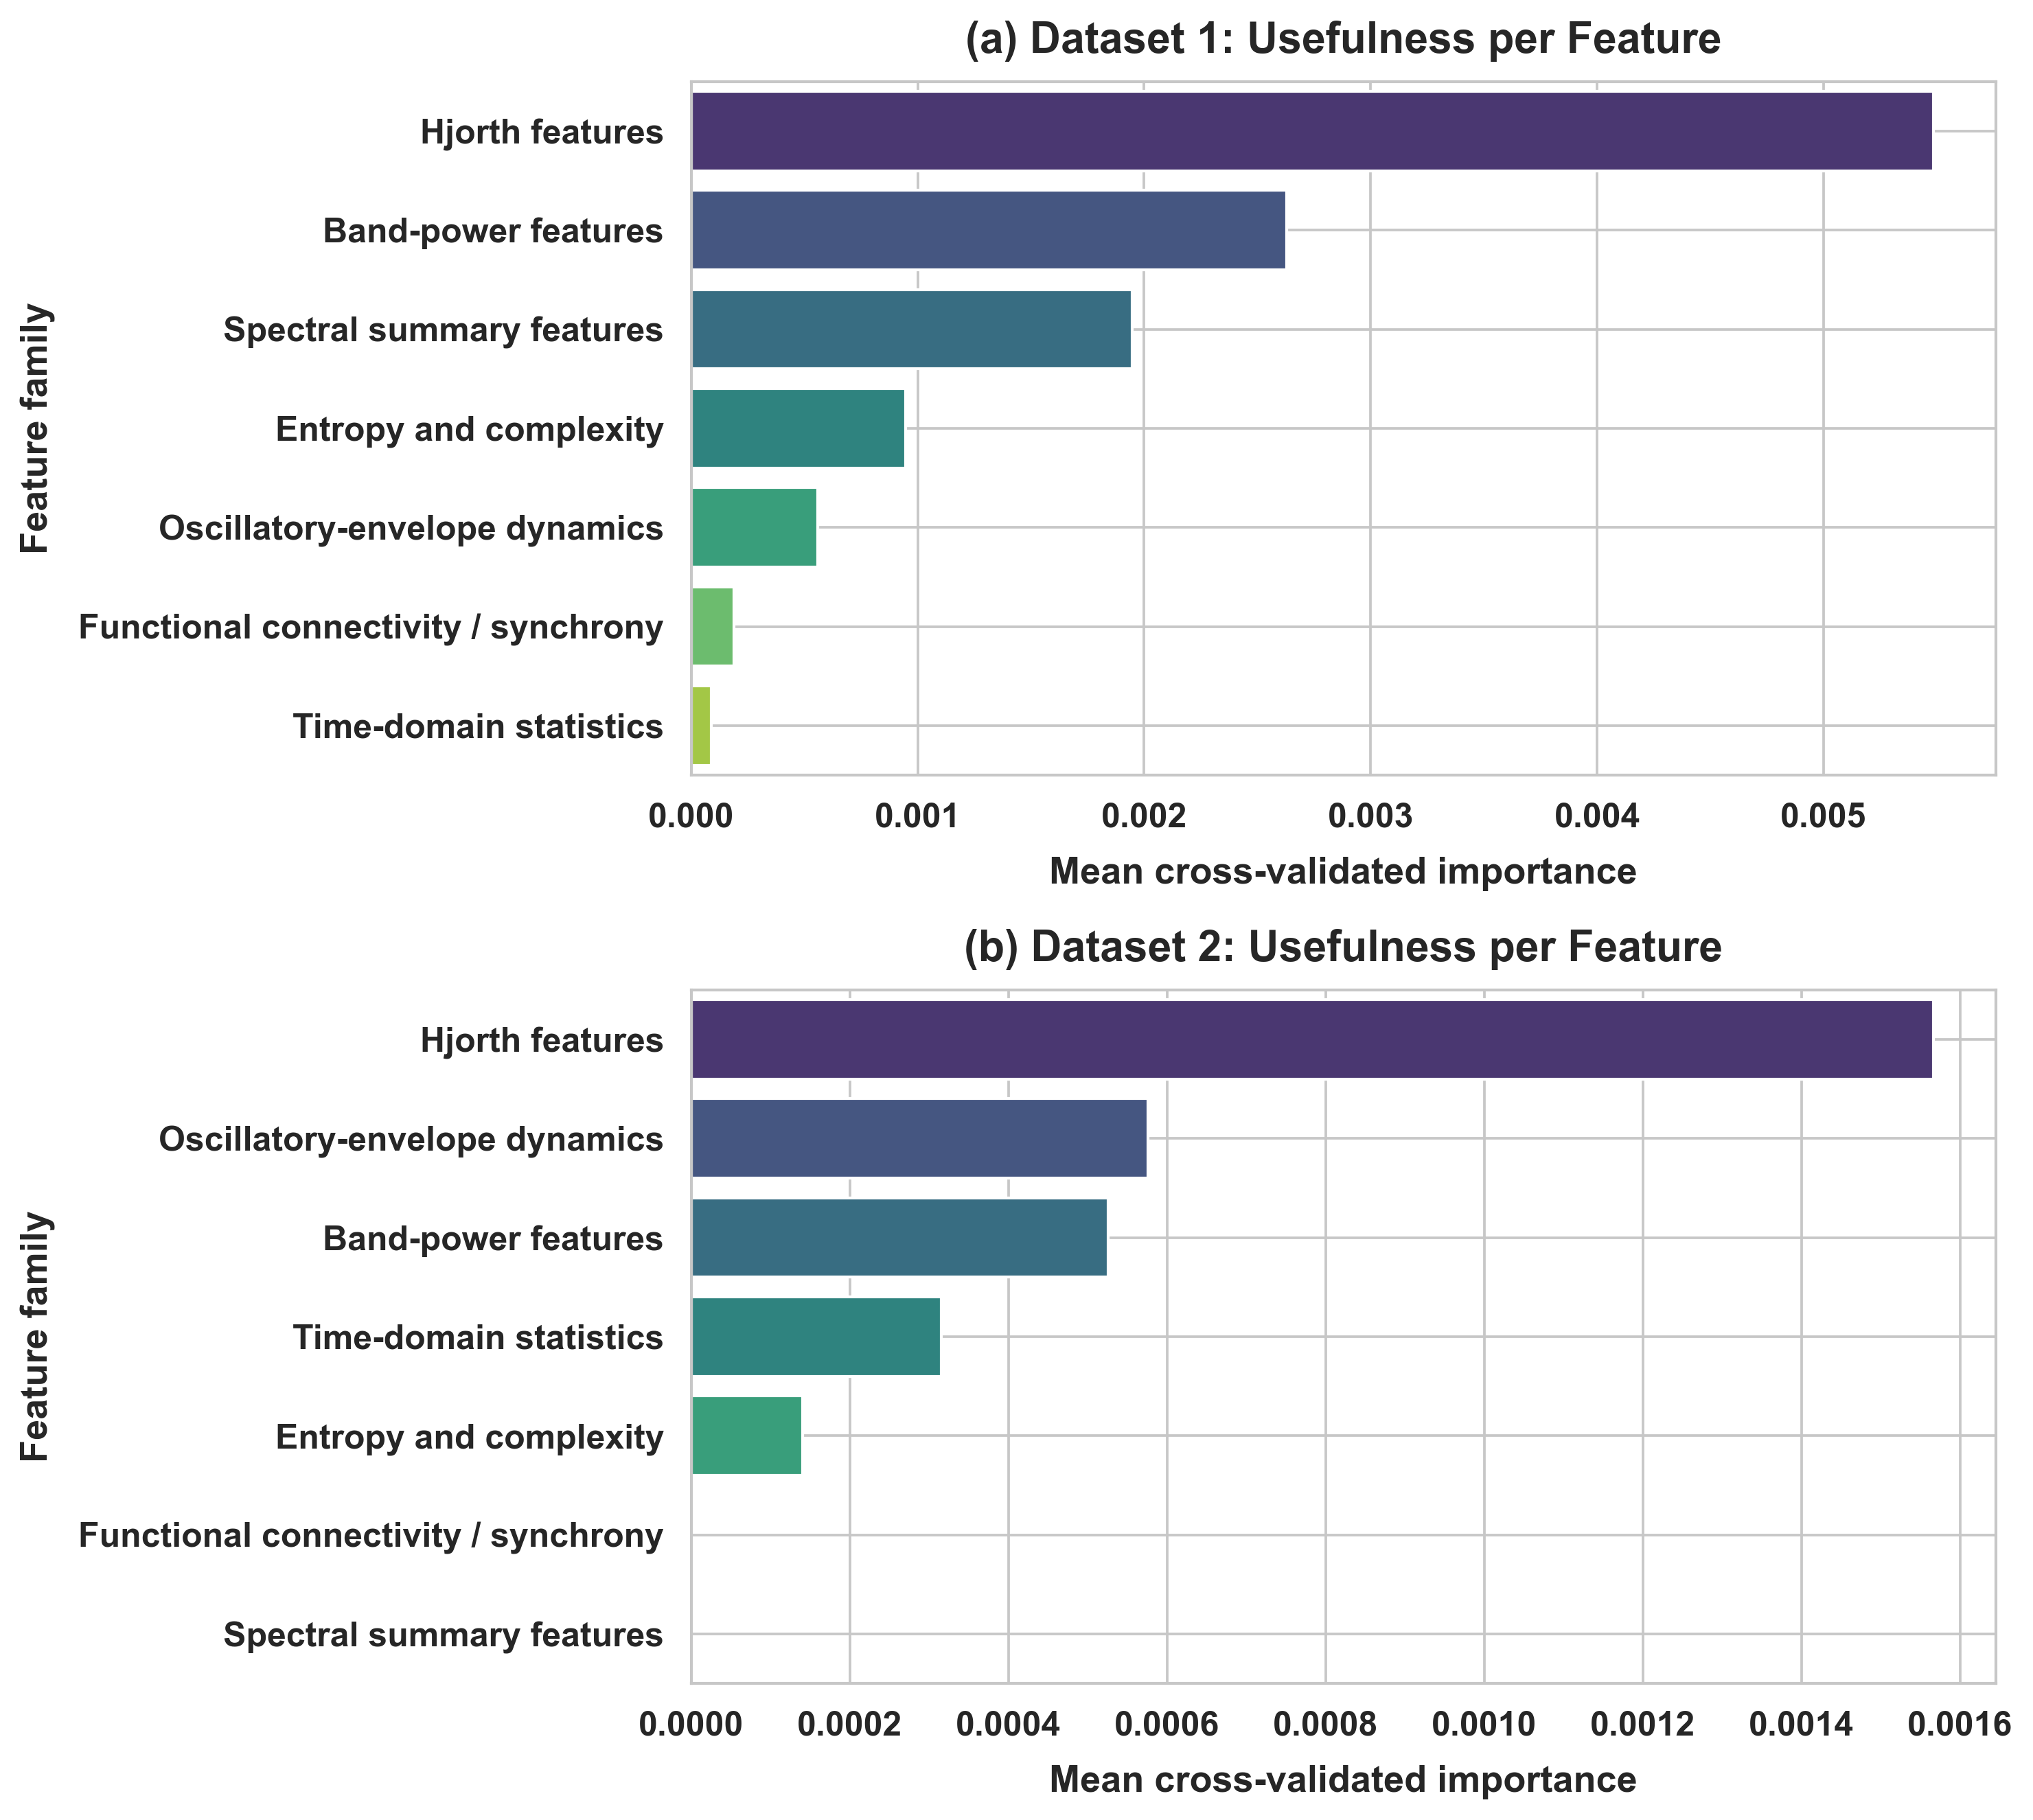
\includegraphics[width=\linewidth]{fig1.png}
    \caption{Feature family comparison for (a) Dataset~1 and (b) Dataset~2.}
    \label{fig:feature_family}
\end{figure}

\subsection{Frequency-Band and Temporal Analysis}

\begin{figure*}[t]
    \centering
    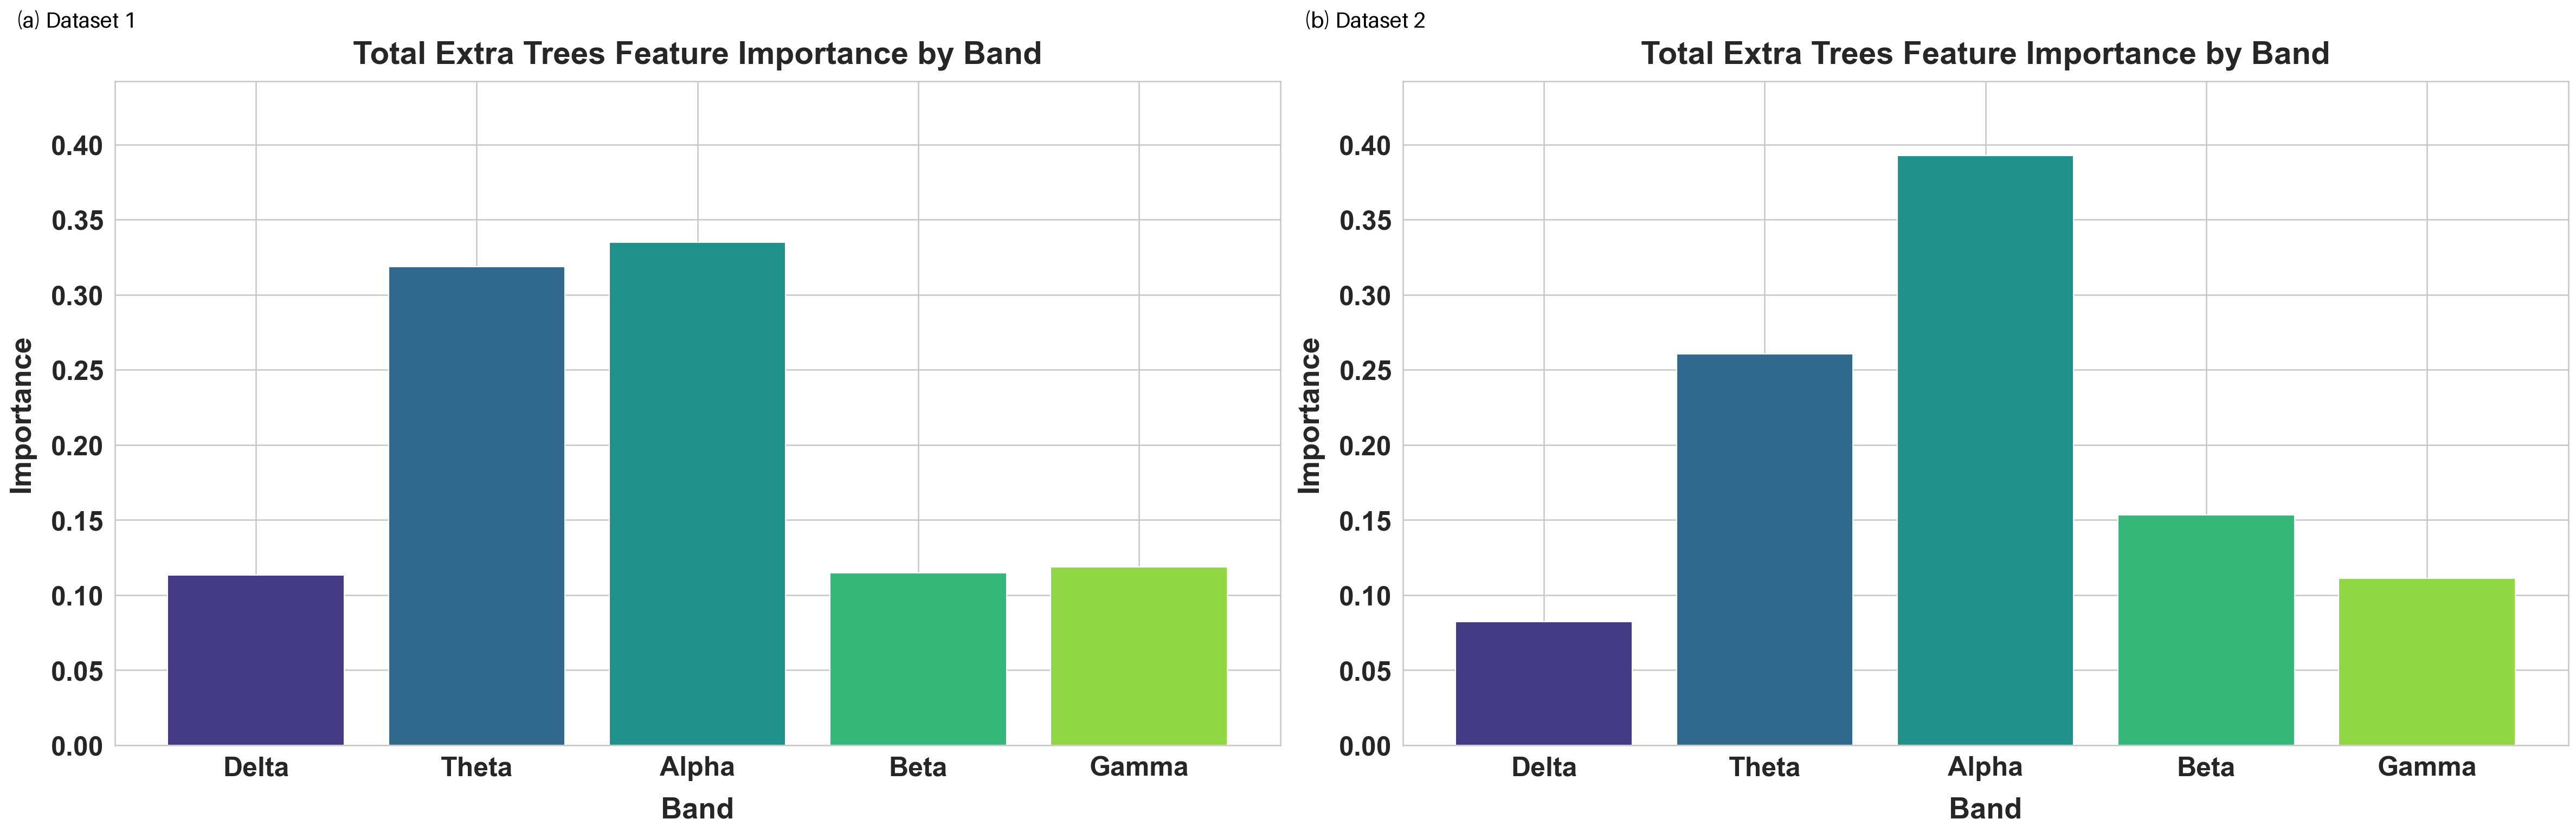
\includegraphics[width=\linewidth,height=4.3cm,keepaspectratio]{fig2.png}
    \caption{Total feature importance across frequency bands for (a) Dataset~1 and
    (b) Dataset~2.}
    \label{fig:band_importance}
\end{figure*}

\textcolor{blue}{Fig.~\ref{fig:band_importance} illustrates the total cross-validated feature importance ($I_b^{\mathrm{total}}$) across individual frequency bands. In Dataset~1, $\alpha$ ($33.50\%$) and $\theta$ ($31.85\%$) contribute the highest total importance, jointly accounting for over $65\%$ of the aggregate feature contribution, while $\gamma$ ($11.87\%$), $\beta$ ($11.47\%$), and $\delta$ ($11.32\%$) exhibit roughly equal secondary contributions. In Dataset~2, a consistent dominance of low-frequency oscillations is observed across both raw and artifact-cleaned EEG, with $\alpha$ providing the highest total importance ($40.94\%$ raw, $39.26\%$ cleaned), followed by $\theta$ ($25.62\%$ raw, $26.07\%$ cleaned) and $\beta$ ($14.91\%$ raw, $15.34\%$ cleaned), whereas $\gamma$ ($10.69\%\text{--}11.10\%$) and $\delta$ ($7.83\%\text{--}8.22\%$) contribute smaller aggregate shares. These findings demonstrate that canonical low-frequency rhythms ($\alpha$ and $\theta$) dominate aggregate tree-based feature contributions across both recording configurations, while higher-frequency and $\delta$ activity provide supplementary discriminative information.}

\begin{figure*}[t]
    \centering
    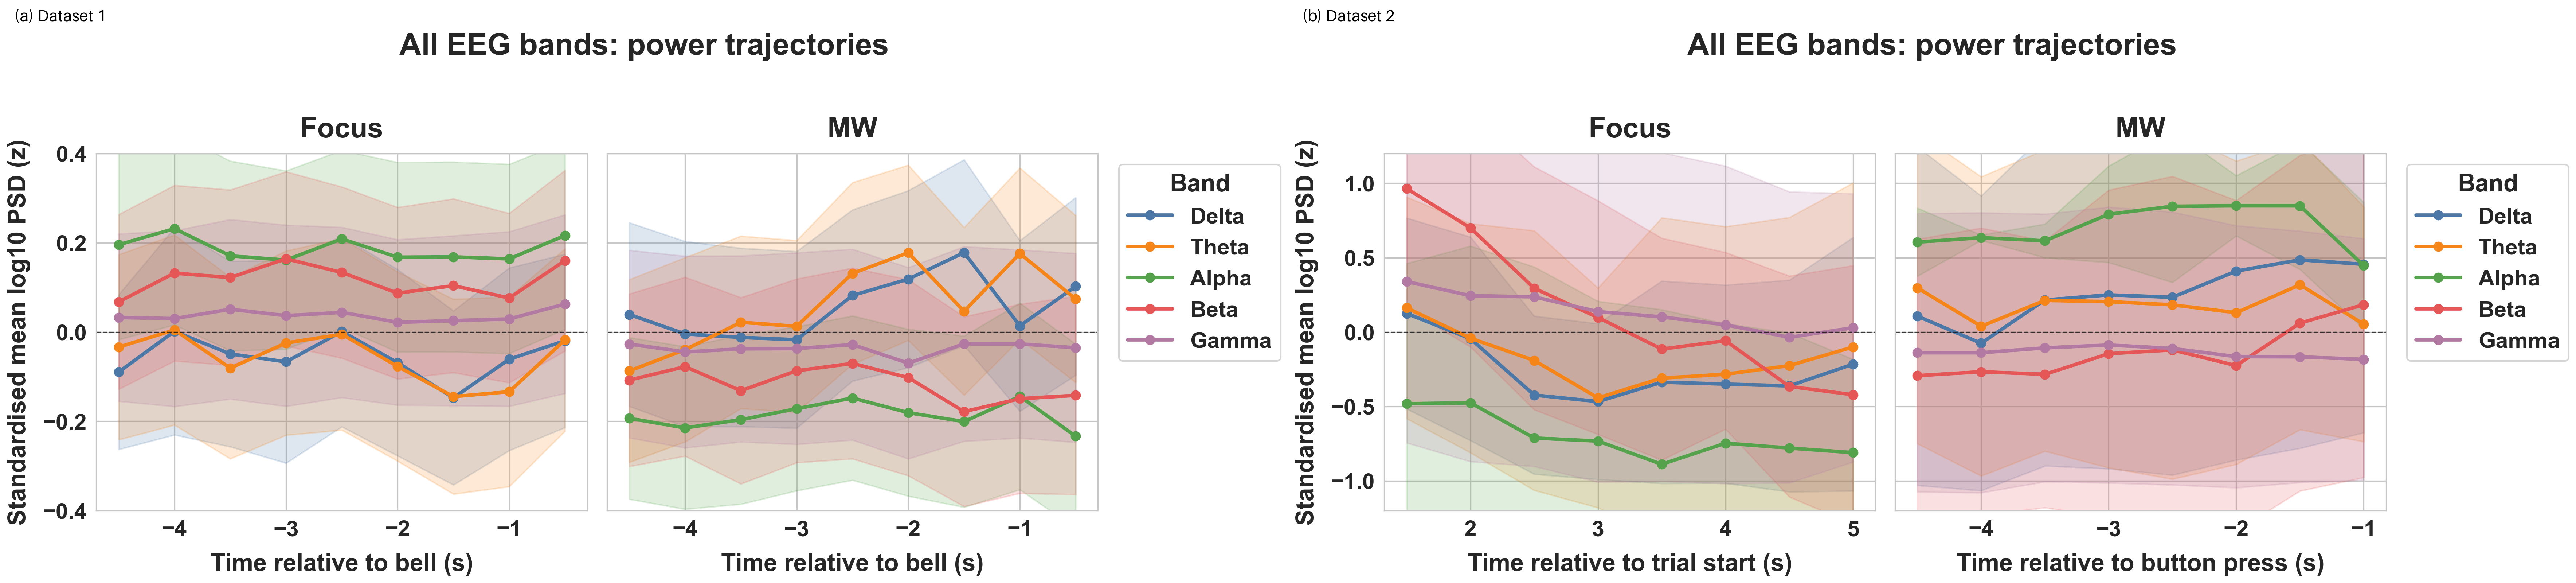
\includegraphics[width=\textwidth,height=4.1cm,keepaspectratio]{fig3.png}
    \caption{Band power trajectories of EEG bands for (a) Dataset~1 and
    (b) Dataset~2.}
    \label{fig:power_trajectories}
\end{figure*}
\textcolor{blue}{Similarly, Fig.~\ref{fig:power_trajectories} illustrates within-epoch spectral trajectories across states. $\theta$ power was significantly higher during MW than Focus across both datasets ($\hat{\beta}=+0.0548$, $z=2.0962$, $p=0.0361$ in Dataset~1; $\hat{\beta}=+0.0333$, $z=5.6970$, $p=1.22\times10^{-8}$ in Dataset~2), with Dataset~1 additionally displaying significant within-epoch accumulation during MW (slope $=+0.0069\,\text{s}^{-1}$, $z=2.0638$, $p=0.0390$).}
\textcolor{blue}{A consistent pattern emerged for $\delta$ activity: mean $\delta$ power exhibited positive MW elevation across both datasets ($\hat{\beta}=+0.0435$ and $+0.0830\,\log_{10}(\mu\text{V}^{2}/\text{Hz})$ for Datasets~1 and~2, respectively). Moreover, $\delta$ power increased progressively over time during MW (slopes $+0.0040\,\text{s}^{-1}$ in Dataset~1 and $+0.0182\,\text{s}^{-1}$ in Dataset~2, the latter $z=3.6422$, $p=2.70\times 10^{-4} < 0.001$), reflecting gradual vigilance degradation.}
\textcolor{blue}{Temporal analysis also revealed critical dynamics masked by static band averages. While mean $\beta$ power was significantly lower during MW in Dataset~1 ($\hat{\beta}=-0.0877$, $z=-2.5835$, $p=0.0098$) but non-significant in Dataset~2 ($\hat{\beta}=-0.0099$, $p=0.5220$), Dataset~2 exhibited strongly divergent within-epoch $\beta$ trajectories: decreasing precipitously during Focus (slope $=-0.0243\,\text{s}^{-1}$, $z=-28.97$, $p=1.42\times10^{-184}$) but increasing during MW (slope $=+0.0088\,\text{s}^{-1}$, $z=1.9680$, $p=0.0491$). Furthermore, mean $\gamma$ power was suppressed during MW across both datasets ($\hat{\beta}=-0.0505$, $p=0.1550$ in Dataset~1; $\hat{\beta}=-0.0342$, $p=0.1199$ in Dataset~2), reflecting electrophysiological evidence for sensory decoupling. In contrast, $\alpha$ activity exhibited notable paradigm-dependent divergence: mean $\alpha$ power was reduced during MW in Dataset~1 ($\hat{\beta}=-0.1211$, $p=0.0832$), but significantly elevated during MW in Dataset~2 ($\hat{\beta}=+0.1127$, $z=2.1040$, $p=0.0354$), reflecting task-specific sensory gating and cortical idling that are fully visible in the temporal trajectories of Fig.~\ref{fig:power_trajectories}.} 
\textcolor{blue}{These findings indicate that MW-related EEG differences are not restricted to static band-power changes; temporal evolution within an epoch provides additional state-discriminative information.}

\subsection{Feature and Frequency-Band Ablation Analysis}
\textcolor{blue}{Table~\ref{tab:ablation_comparison} summarizes the systematic ablation results across feature families, scalp regions, and frequency bands evaluated using SVM on raw EEG under subject-session grouped cross-validation (\texttt{StratifiedGroupKFold}). Both feature-family and frequency-band ablations were executed on the complete multi-domain feature representation, sharing the common baseline of 61.40\% accuracy (57.30\% F1, AUC 65.87\%) in Dataset~1 and 68.39\% accuracy (59.39\% F1, AUC 77.53\%) in Dataset~2. Omitting spectral features produced significant performance degradation in both datasets (dropping to 60.70\% accuracy with AUC 64.86\% in Dataset~1, and 60.94\% accuracy with AUC 70.31\% in Dataset~2), confirming the indispensable role of oscillatory dynamics for robust discrimination. When isolating individual feature families, spectral features yielded the highest isolated performance across both datasets (61.70\% accuracy, AUC 65.06\% in Dataset~1; 65.52\% accuracy, AUC 75.77\% in Dataset~2), closely matched by time-domain descriptors in Dataset~2 (65.43\% accuracy). In contrast, isolated time-domain features in Dataset~1 (57.70\%) and isolated Hjorth in Dataset~2 (52.63\%) yielded the lowest isolated accuracies.}

\textcolor{blue}{Spatial and frequency-band ablations across the full feature space revealed pronounced paradigm-specific dynamics. Spatial ablation demonstrated that central and temporal channels were most vital in Dataset~1 (omission dropping accuracy to 57.10\%, AUC 63.22\%), whereas posterior channels dominated in Dataset~2 (only posterior yielding 73.83\% accuracy, AUC 78.38\%). In frequency-band ablation, multi-domain features provided high resilience in Dataset~1, with isolated $\beta$ activity offering the strongest single-band performance (59.00\% accuracy, AUC 60.35\%), while omitting $\theta$ or $\alpha$ preserved performance at 62.40\% accuracy. In Dataset~2, $\alpha$ activity proved decisively to be the most critical band: omitting $\alpha$ caused the steepest degradation among all bands (dropping to 63.42\% accuracy, 50.20\% F1, AUC 66.03\%), whereas retaining only $\alpha$ activity preserved 67.81\% accuracy (63.01\% F1, AUC 71.25\%)—nearly matching the full-feature baseline single-handedly. Conversely, omitting $\gamma$ in Dataset~2 improved accuracy to 71.54\% (AUC 79.99\%), indicating that pruning high-frequency muscle and noise artifacts enhances out-of-session generalization. These full-representation ablation results confirm that while discriminative information is distributed across multi-domain descriptors, spatial and band dependencies are critically governed by paradigm-specific cognitive demands.}

\begin{table}[h]
\centering
\caption{Ablation analysis using SVM on raw EEG. \textcolor{blue}{Where variants diverge across datasets, they are reported as (Dataset~1 / Dataset~2).}}
\label{tab:ablation_comparison}
\resizebox{\linewidth}{!}{%
\begin{tabular}{llrrr|rrr}
\toprule
& & \multicolumn{3}{c|}{Dataset 1} & \multicolumn{3}{c}{Dataset 2} \\
Category & Variant & Acc. & F1 & AUC & Acc. & F1 & AUC \\
\midrule
Baseline
& Full feature set
& \textcolor{blue}{61.40} & \textcolor{blue}{57.30} & \textcolor{blue}{65.87}
& 68.39 & 59.39 & 77.53 \\
\midrule
\multirow{2}{*}{\textcolor{blue}{Feature family (Omission)}}
& Best omission (\textcolor{blue}{Omit Hjorth / Omit Hjorth})
& \textcolor{blue}{61.80} & \textcolor{blue}{57.27} & \textcolor{blue}{66.00}
& 68.77 & 61.12 & 76.72 \\
& Most damaging omission (Omit Spectral)
& \textcolor{blue}{60.70} & \textcolor{blue}{56.57} & \textcolor{blue}{64.86}
& \textcolor{blue}{60.94} & \textcolor{blue}{53.26} & \textcolor{blue}{70.31} \\
\midrule
\multirow{2}{*}{\textcolor{blue}{Feature family (Isolation)}}
& Best isolated (\textcolor{blue}{Only Spectral / Only Spectral})
& \textcolor{blue}{61.70} & \textcolor{blue}{57.40} & \textcolor{blue}{65.06}
& 65.52 & 57.78 & 75.77 \\
& Most damaging isolated (\textcolor{blue}{Only Time-Domain / Only Hjorth})
& \textcolor{blue}{57.70} & \textcolor{blue}{52.74} & \textcolor{blue}{62.24}
& 52.63 & 37.22 & 56.27 \\
\midrule
\multirow{2}{*}{\textcolor{blue}{Scalp region (Omission)}}
& \textcolor{blue}{Best omission (Omit Posterior / Omit Frontal)}
& \textcolor{blue}{62.70} & \textcolor{blue}{58.04} & \textcolor{blue}{67.30}
& \textcolor{blue}{67.72} & \textcolor{blue}{55.53} & \textcolor{blue}{78.55} \\
& \textcolor{blue}{Most damaging omission (Omit Central \& Temp. / Omit Posterior)}
& \textcolor{blue}{57.10} & \textcolor{blue}{53.01} & \textcolor{blue}{63.22}
& \textcolor{blue}{66.19} & \textcolor{blue}{55.75} & \textcolor{blue}{72.93} \\
\midrule
\multirow{2}{*}{\textcolor{blue}{Frequency band (Omission)}}
& Best omission (\textcolor{blue}{Omit Theta / Omit Gamma})
& \textcolor{blue}{62.40} & \textcolor{blue}{58.59} & \textcolor{blue}{65.82}
& \textcolor{blue}{71.54} & \textcolor{blue}{66.37} & \textcolor{blue}{79.99} \\
& Most damaging omission (\textcolor{blue}{Omit Delta / Omit Alpha})
& \textcolor{blue}{61.40} & \textcolor{blue}{57.77} & \textcolor{blue}{65.90}
& \textcolor{blue}{63.42} & \textcolor{blue}{50.20} & \textcolor{blue}{66.03} \\
\midrule
\multirow{2}{*}{\textcolor{blue}{Frequency band (Isolation)}}
& Best isolated (\textcolor{blue}{Only Beta / Only Alpha})
& \textcolor{blue}{59.00} & \textcolor{blue}{55.04} & \textcolor{blue}{60.35}
& \textcolor{blue}{67.81} & \textcolor{blue}{63.01} & \textcolor{blue}{71.25} \\
& Most damaging isolated (\textcolor{blue}{Only Alpha / Only Theta})
& \textcolor{blue}{54.90} & \textcolor{blue}{53.07} & \textcolor{blue}{58.27}
& \textcolor{blue}{53.01} & \textcolor{blue}{49.69} & \textcolor{blue}{57.57} \\
\bottomrule
\end{tabular}%
}
\end{table}

\section{Conclusion}

\textcolor{blue}{This study presented an integrated multi-domain EEG framework characterizing mind wandering across two datasets differing in montage density and task paradigm. We demonstrated that discriminative information is distributed across complementary representations: Hjorth parameters exhibit exceptional information density per feature, canonical low-frequency ($\alpha$ and $\theta$) oscillations dominate total spectral contributions, and within-epoch temporal trajectories reveal critical neural dynamics masked by static averages. Systematic ablation confirmed that the most informative feature family and frequency band varied across paradigms, while integrated multi-domain representations enabled linear models to match deep architectures at up to 88.06\% accuracy. These findings confirm that MW-related neural signatures are shaped by paradigm-dependent cognitive processes and underscore the necessity of multi-dimensional characterization over single-domain approaches.}

\section*{Acknowledgment}
This research was supported by the Anusandhan National Research Foundation (ANRF), Department of Science and Technology, Government of India, under grant number ANRF/ECRG/2024/004043/ENS.

\bibliographystyle{IEEEtran}
\bibliography{references}
\end{document}